\documentclass[11pt,a4paper]{article}
\usepackage[margin=1.9cm]{geometry}
\usepackage[T1]{fontenc}
\usepackage{lmodern}
\usepackage{xcolor}
\usepackage{graphicx}
\usepackage{booktabs}
\usepackage{longtable}
\usepackage{listings}
\usepackage{hyperref}
\usepackage{fancyhdr}
\hypersetup{colorlinks=true,urlcolor=blue!60!black,linkcolor=blue!60!black}
\pagestyle{fancy}\fancyhf{}\lhead{Boeing 747-8 RL Takeoff}\rhead{Project handover}\cfoot{\thepage}
\lstset{basicstyle=\ttfamily\small,breaklines=true,frame=single,backgroundcolor=\color{gray!7}}
\title{Teaching a Giant Airliner to Take Off\\\large A Friendly Guide to the Boeing 747-8 Reinforcement-Learning Project}
\author{Project handover report}\date{2026-10-08 11:34 Maroc}
\begin{document}\maketitle
\begin{center}\fcolorbox{blue!45!black}{blue!5}{\parbox{0.88\linewidth}{\textbf{One sentence:} A simulated pilot learns to control throttle, elevator, aileron and rudder so a research approximation of a Boeing 747-8 can perform a clean, stable takeoff in many changing conditions.}}\end{center}
\tableofcontents\clearpage
\section{The one-minute story}
Imagine a student pilot practising the same takeoff thousands of times. The pilot sees 27 instrument values, moves four controls, and receives a score. Good actions earn points; dangerous or messy actions lose points. After every attempt, the SAC algorithm adjusts a neural network so the next attempt can be better. A hand-written ``teacher pilot'' supplies good examples so learning does not start from pure chaos.
\begin{figure}[h]\centering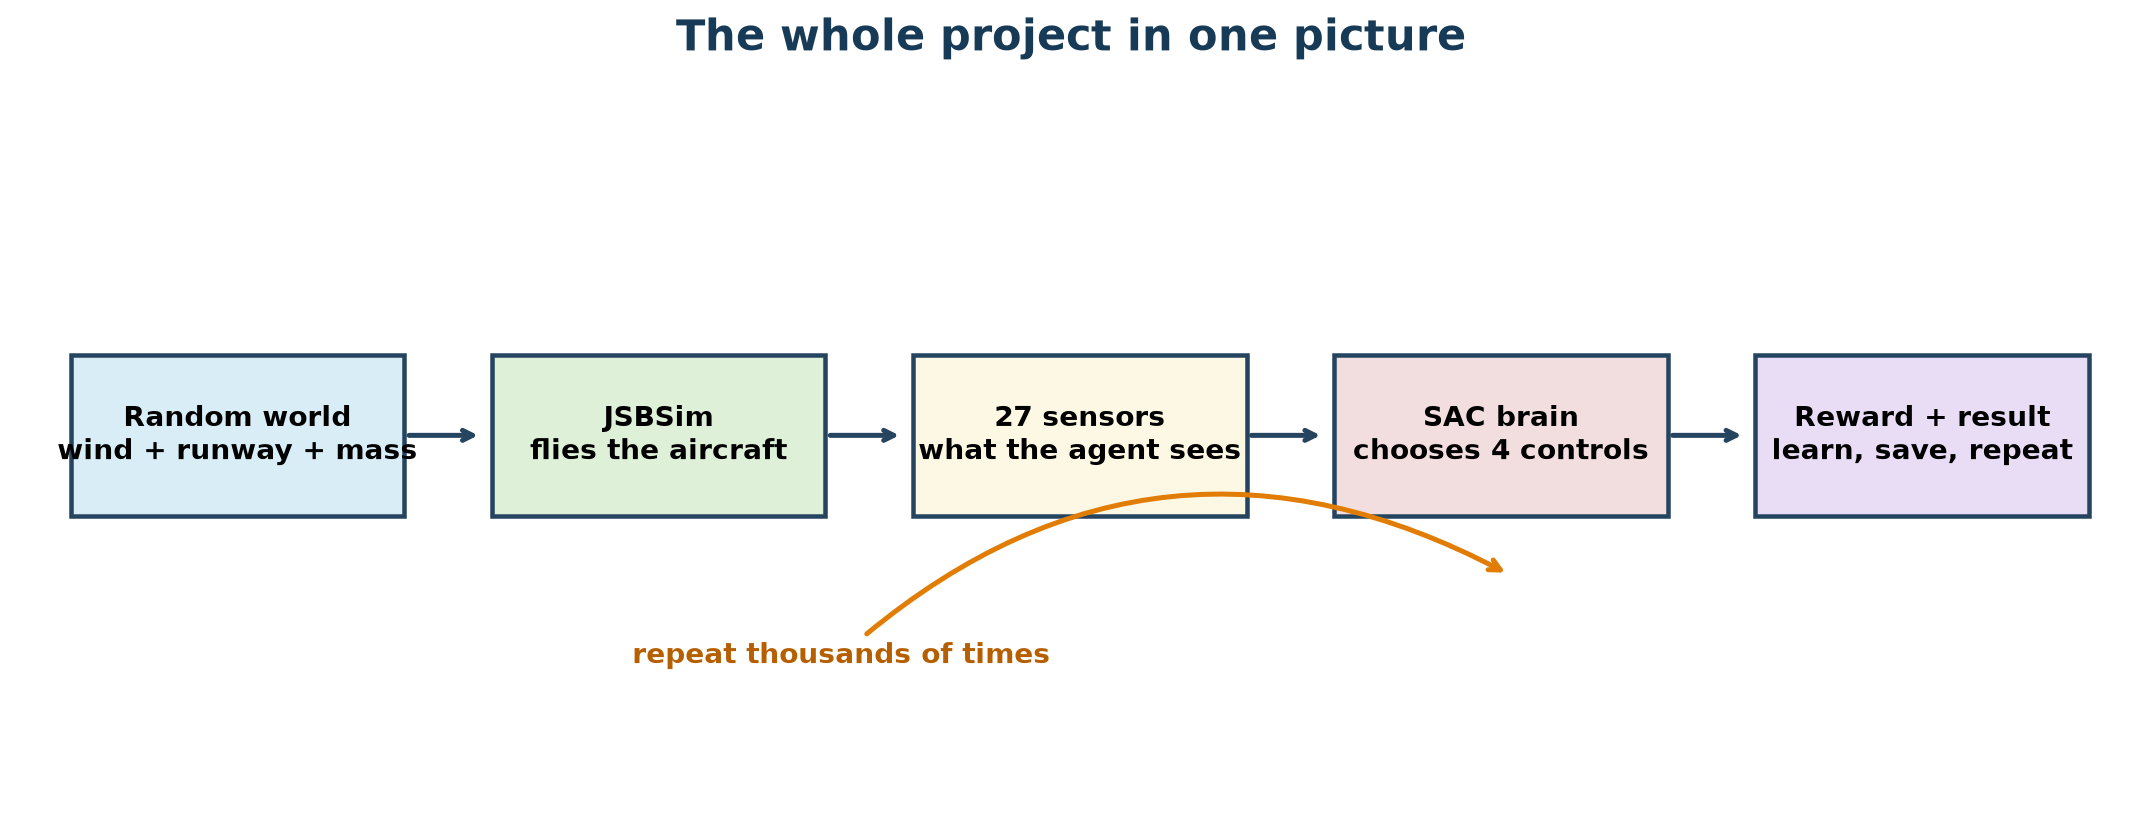
\includegraphics[width=\linewidth]{assets/project_flow.png}\caption{The learning loop. Remember: \textbf{world - physics - sensors - brain - score}.}\end{figure}
\section{What success means}
The goal is not just ``leave the ground.'' The aircraft must accelerate, stay near the centerline, rotate around the estimated rotation speed, climb past 1,000 ft AGL, remain stable for five seconds, and keep a cleanliness score of at least 0.5.
\begin{figure}[h]\centering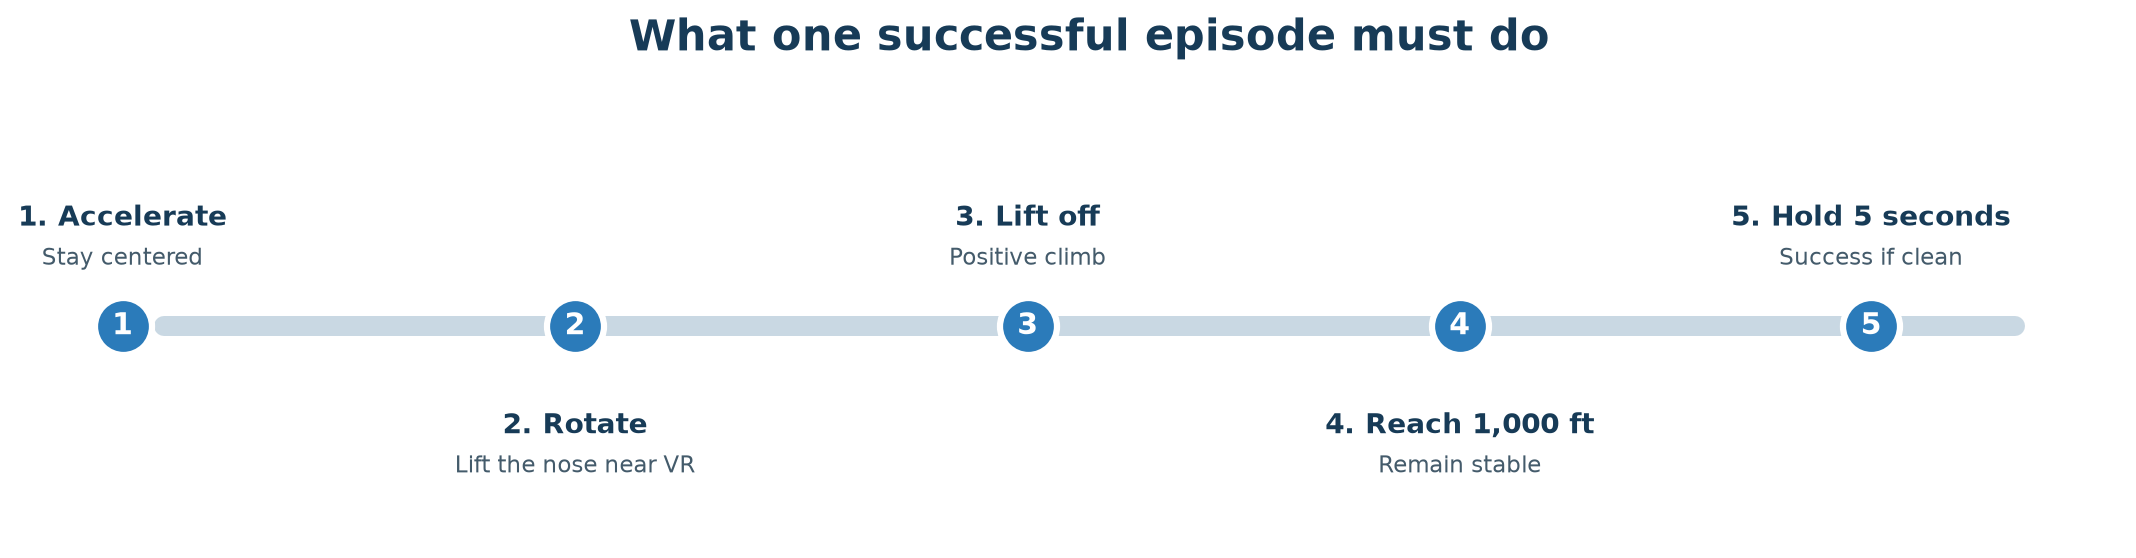
\includegraphics[width=\linewidth]{assets/takeoff_story.png}\caption{A complete successful episode.}\end{figure}
\section{The cast of characters}
\begin{longtable}{p{0.22\linewidth}p{0.70\linewidth}}\toprule
\textbf{Word} & \textbf{Plain-English meaning}\\\midrule
Agent & The neural-network pilot.\\
Environment & The practice world that runs the flight and judges it.\\
Observation & The 27-number instrument panel presented to the agent.\\
Action & Four commands: throttle, elevator, aileron and rudder.\\
Reward & The score that says ``more like this'' or ``less like this.''\\
Episode & One takeoff attempt, from the runway start to success or failure.\\
Teacher & A conventional hand-tuned controller that demonstrates sensible takeoffs.\\
Curriculum & Five difficulty levels that add harder wind, runway and aircraft conditions.\\
Checkpoint & A saved brain plus replay buffer and training state.\\\bottomrule\end{longtable}
\section{The aircraft: useful, but not a real certified 747-8}
The physics engine is JSBSim. Because no validated JSBSim 747-8 model was found, the project starts from JSBSim's Boeing 747-400 model and replaces a limited set of values with published 747-8 numbers: wingspan, wing area, empty weight, fuel capacity and engine thrust. Aerodynamic tables, inertia, landing gear and many engine details still come from the older 747-400 model. The project therefore labels the aircraft \texttt{7478\_RESEARCH\_APPROXIMATION}. Results are for simulation research only.
\begin{figure}[h]\centering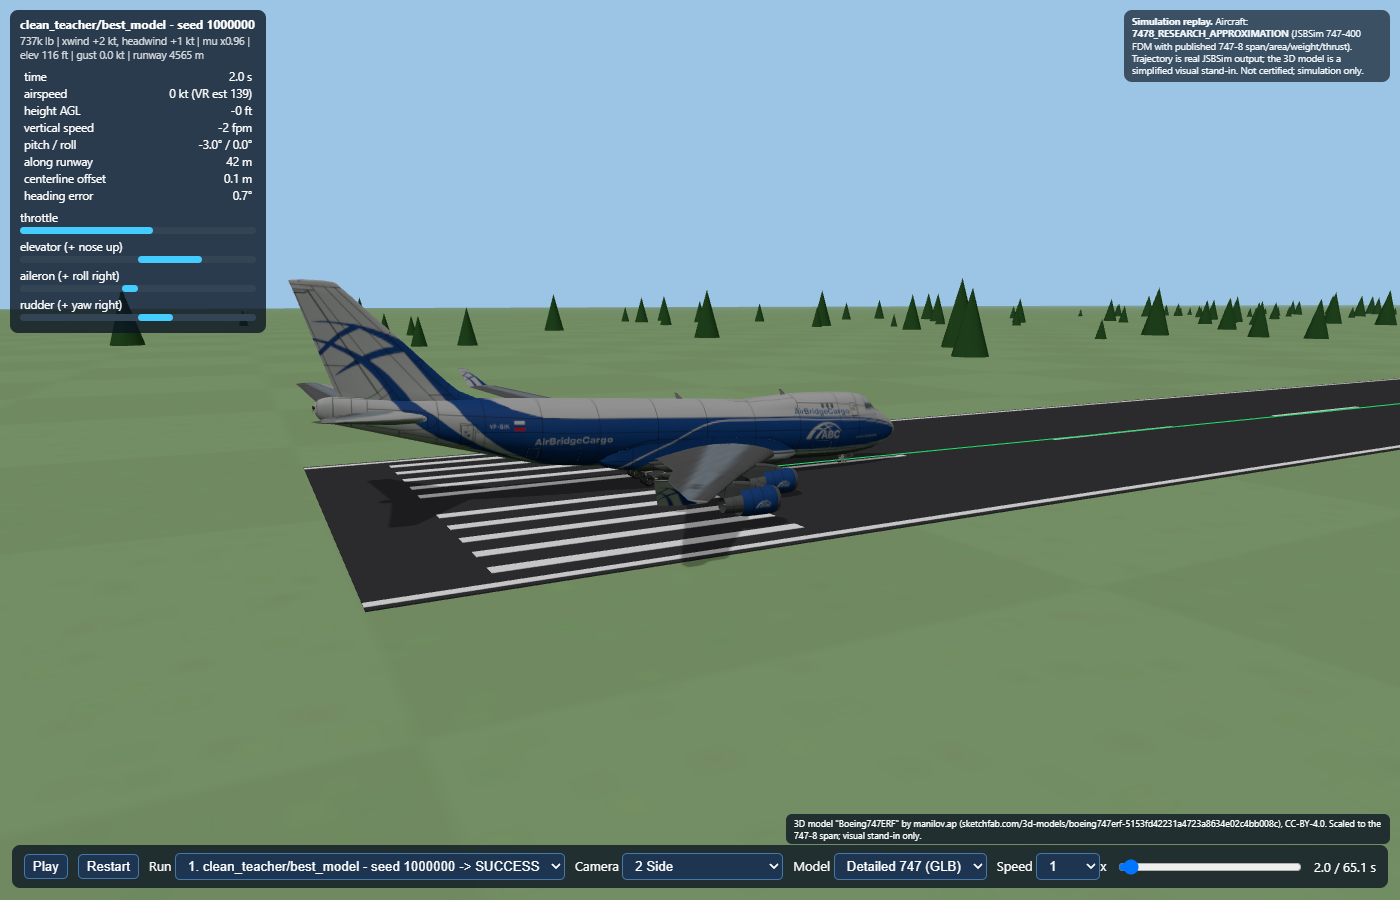
\includegraphics[width=\linewidth]{assets/simulation_3d.png}\caption{The 3D replay viewer. The GLB is a visual stand-in only and does not change the flight physics.}\end{figure}
\section{What the agent sees and controls}
The 27 observations include speed, height, climb rate, pitch, roll, heading, angle of attack, sideslip, body rates, runway errors, distance, wheel contact, actuator positions, engine state, mass, centre of gravity, wind and air-density ratio. Values are normalised and clipped so the neural network receives numbers of a predictable size.

The action vector has four values in $[-1,1]$: throttle, elevator, aileron and rudder. An actuator layer clips invalid commands, rate-limits movement, maps throttle to $[0,1]$, converts signs to JSBSim conventions, and links rudder pedals to nose-wheel steering. The policy acts at 10 Hz; JSBSim runs 12 smaller physics steps at 120 Hz for each policy action.
\section{How the score teaches clean flying}
The reward is a collection of readable terms. Positive terms reward runway progress, centreline tracking, correct heading, acceleration, rotation, climbing, altitude progress, stability and final success. Negative terms penalise time, lateral error, excessive roll/heading/AoA/sideslip, control oscillation, premature rotation and terminal failures. The \texttt{clean} profile adds passenger-comfort terms for tight centreline tracking, low sideways motion, low lateral acceleration, low yaw/roll rates and a cleanliness bonus.

Memorise the rule as \textbf{fast enough, straight enough, smooth enough, stable enough}.
\section{How learning is organised}
The main algorithm is Soft Actor-Critic (SAC), with three 256-unit ReLU layers for actor and critics, a replay buffer of one million transitions and automatic entropy tuning. The teacher dataset is placed into the replay buffer, and behaviour cloning gives the actor a sensible starting point. SAC then continues learning from its own experience.

Curriculum advancement uses deterministic evaluation, never noisy training reward. The threshold is above 80 percent across at least 20 evaluation episodes. Level 1 is gentle; levels 2 and 3 widen the conditions; levels 4 and 5 include stronger wind, shorter or slippery runways, high elevation, gusts and turbulence.
\begin{figure}[h]\centering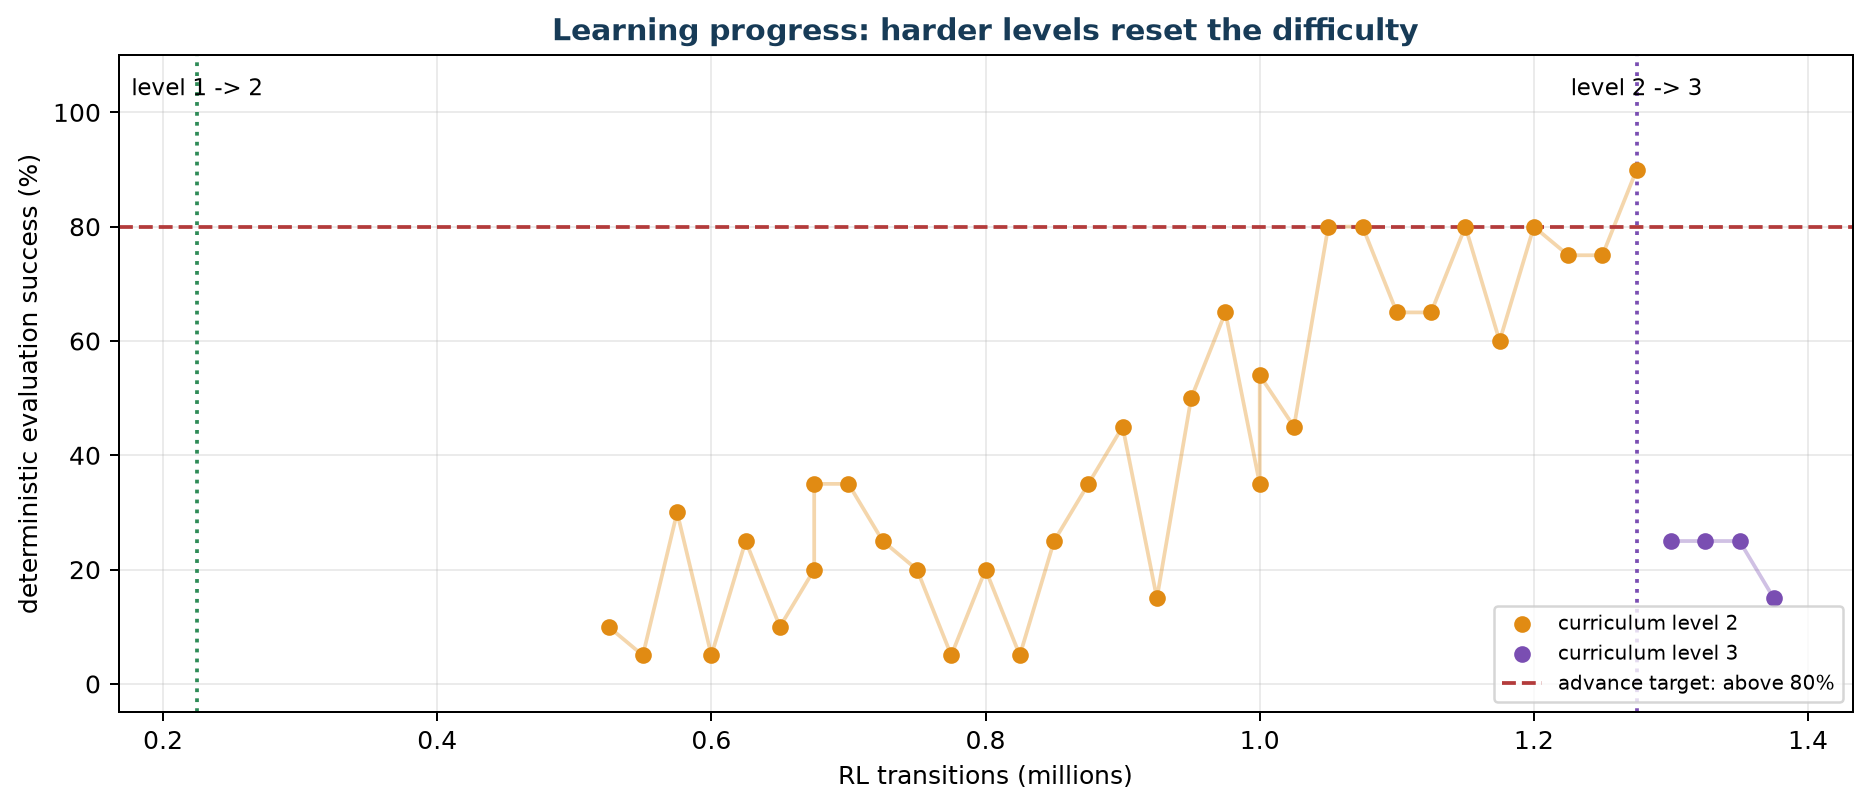
\includegraphics[width=0.96\linewidth]{assets/evaluation_progress.png}\caption{Evaluation success by training step. A drop after a level-up is expected because the exam becomes harder.}\end{figure}
\section{Current stage: 1,386,000 transitions}
The strongest active run is \texttt{clean\_teacher\_lv4}. At this snapshot it has completed 1,386,000 RL transitions, 920 training episodes and 585 training successes. Its rolling success rate over the latest 100 episodes is 42 percent. It moved from level 1 to level 2 at 225,000 transitions, and from level 2 to level 3 at 1,275,000 transitions. The latest deterministic level-3 evaluation is 15 percent over 20 episodes. This means the system has learned convincing behaviour through level 2 and is now adapting to the harder level-3 conditions; it is not yet a final, fully robust policy.

Milestones: first successful training takeoff at 107,676 transitions; 10 percent rolling success at 249,695; 50 percent at 732,075; and 90 percent at 1,106,454 transitions.
\begin{figure}[h]\centering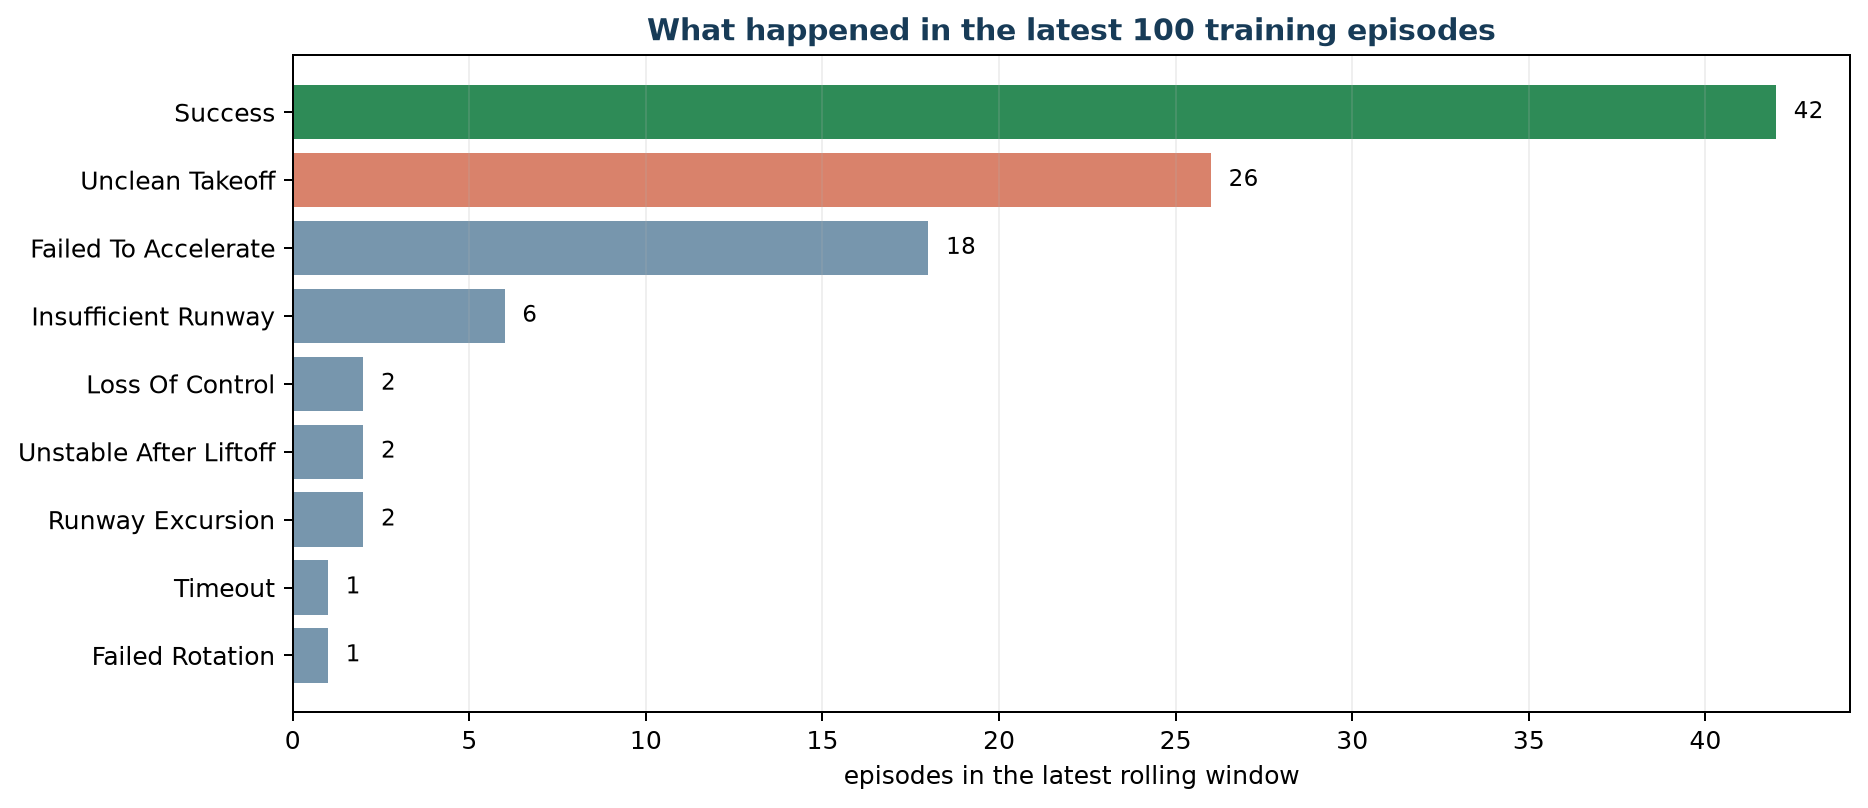
\includegraphics[width=0.92\linewidth]{assets/recent_outcomes.png}\caption{Latest rolling outcomes. ``Unclean takeoff'' means the aircraft reached the goal region but the whole flight was not smooth enough.}\end{figure}
\section{What a good and bad episode look like}
\begin{figure}[h]\centering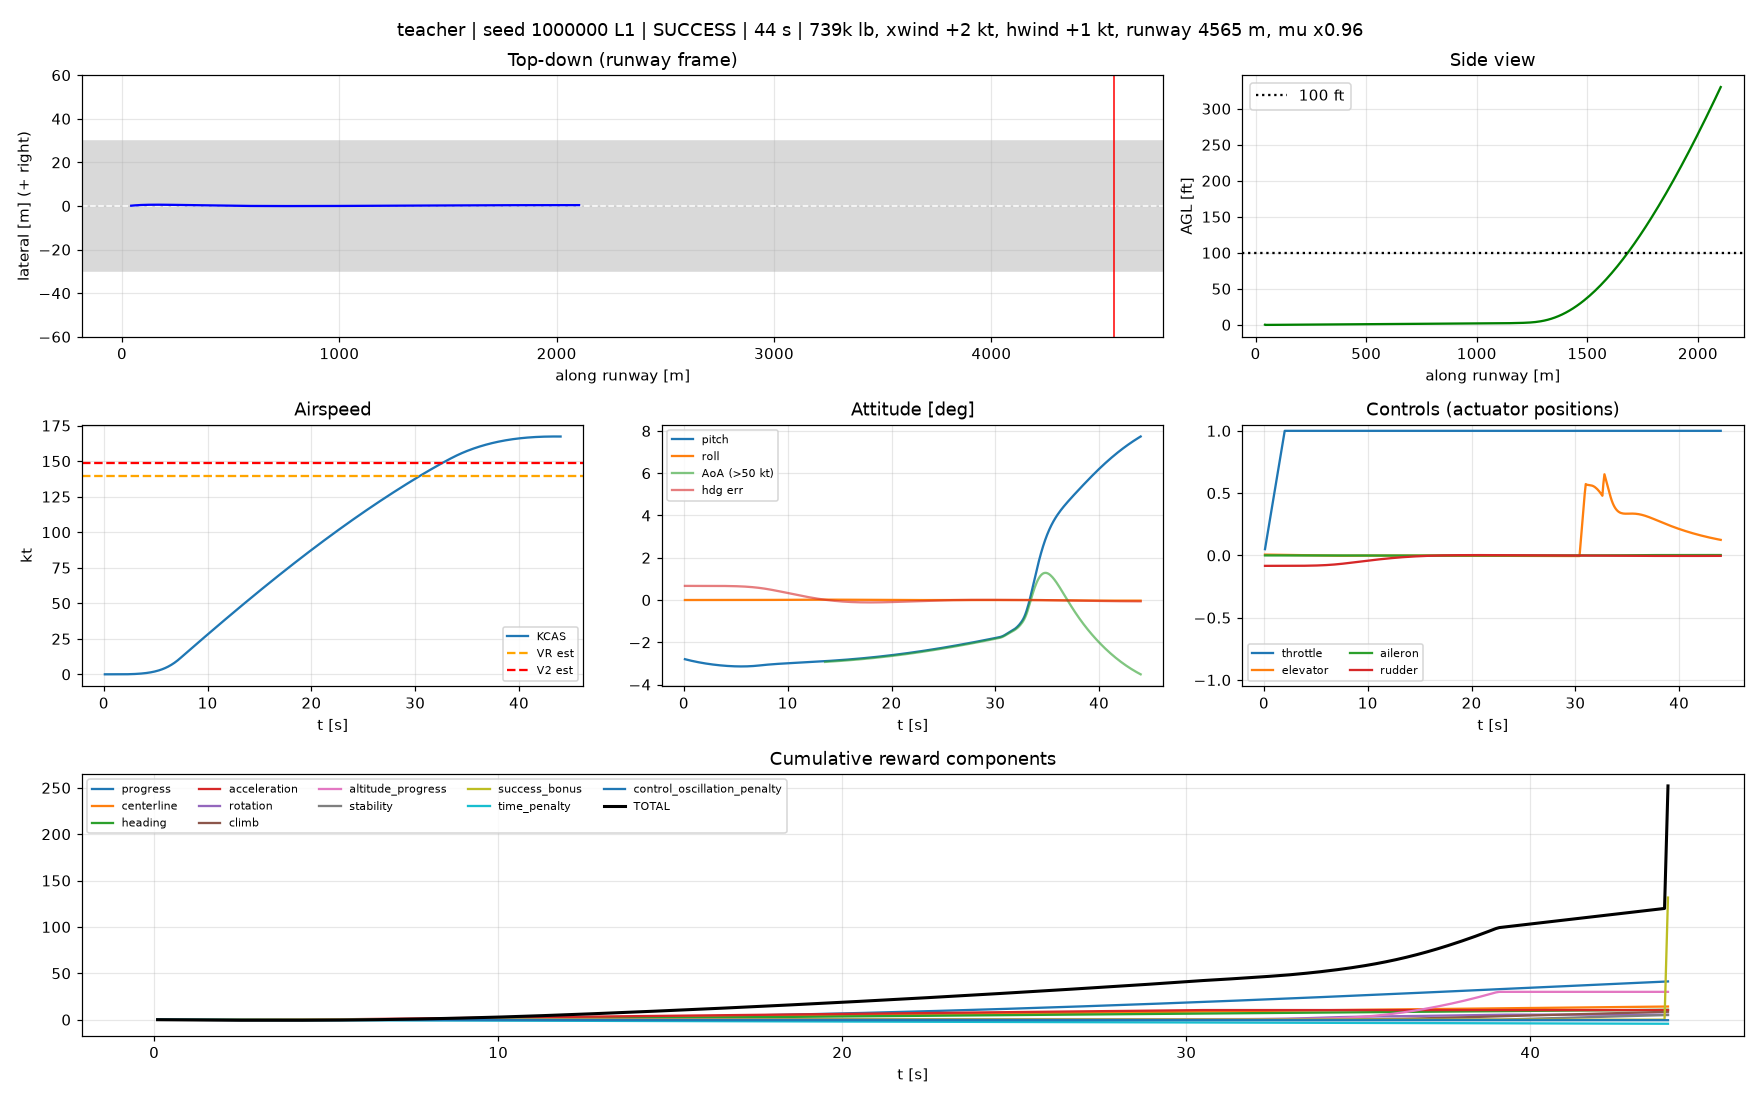
\includegraphics[width=\linewidth]{assets/teacher_success_dashboard.png}\caption{Successful teacher trajectory: centered runway track, smooth rotation and stable climb.}\end{figure}
\begin{figure}[h]\centering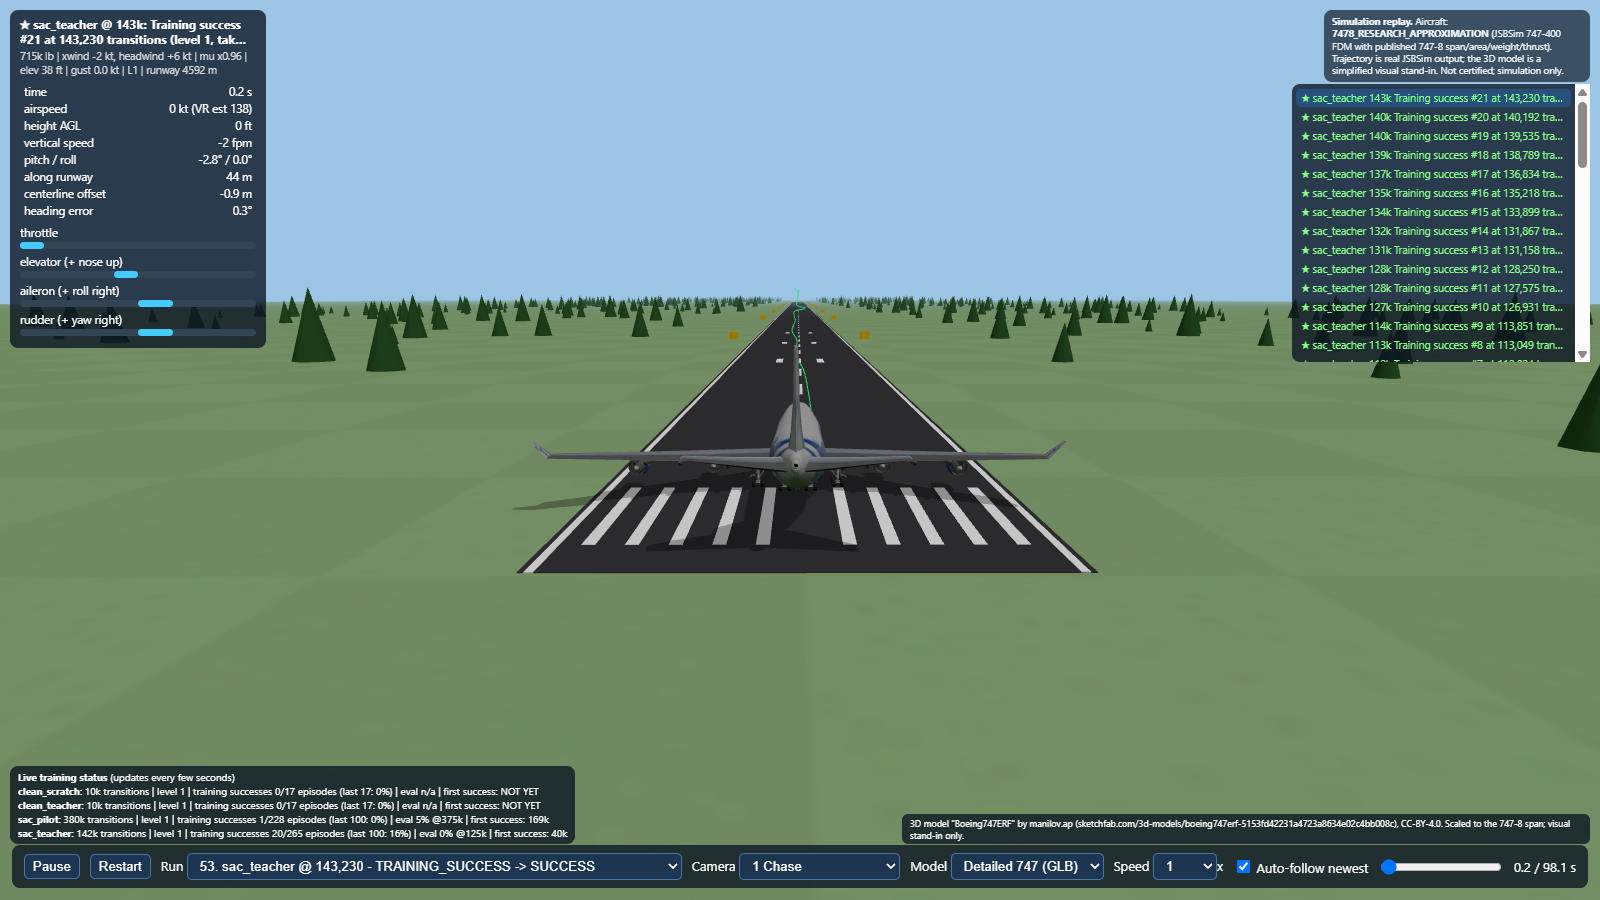
\includegraphics[width=\linewidth]{assets/training_success_3d.png}\caption{A recorded training success in the 3D replay. The green history list confirms repeated successful episodes.}\end{figure}
\begin{figure}[h]\centering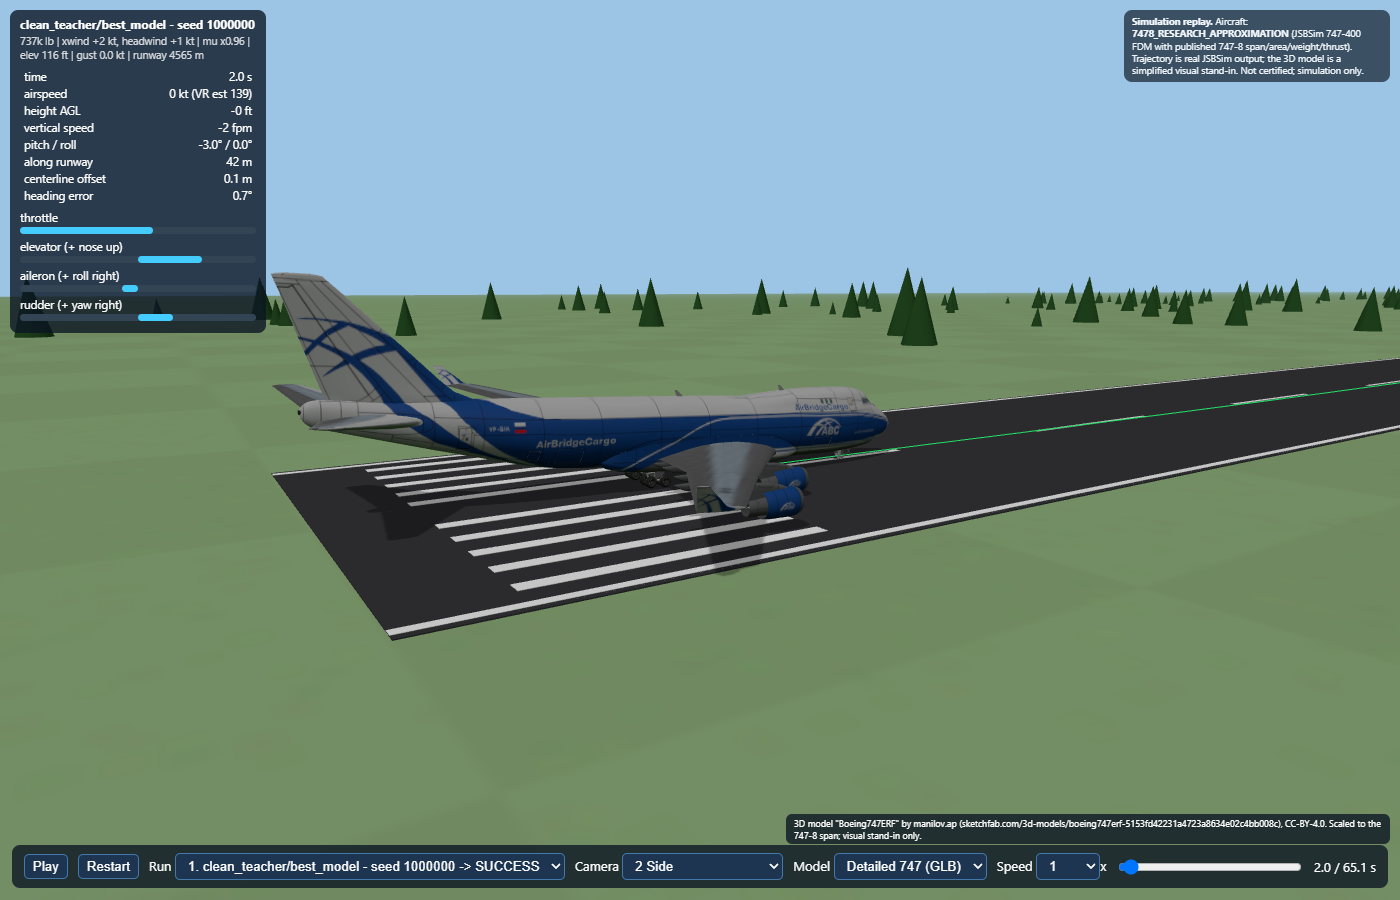
\includegraphics[width=\linewidth]{assets/successful_runway_start_side.png}\caption{Side view of a successful replay at the runway start. Check alignment, wheel contact and heading before judging the later climb.}\end{figure}
\begin{figure}[h]\centering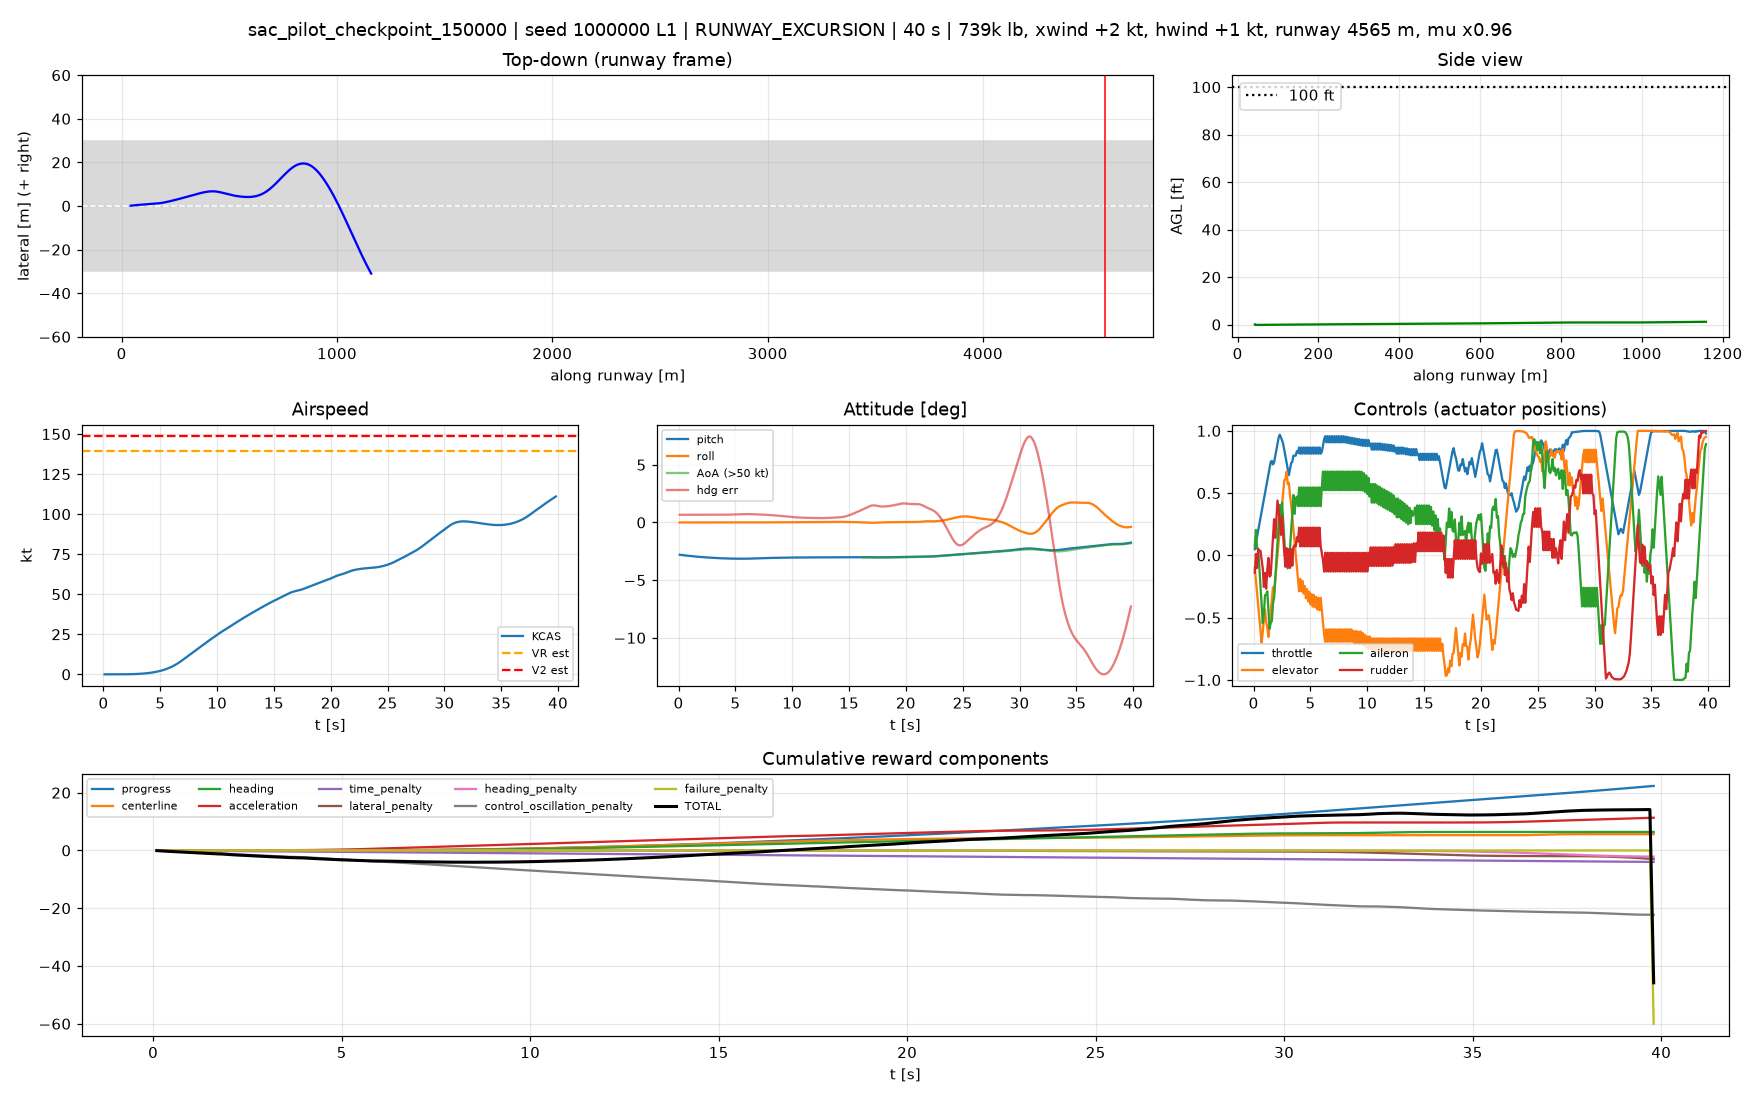
\includegraphics[width=\linewidth]{assets/early_agent_failure.png}\caption{Early learned-policy failure: the aircraft wanders, uses rough controls and exits the runway.}\end{figure}
\section{Project map: where to look}
\begin{longtable}{p{0.24\linewidth}p{0.66\linewidth}}\toprule
\textbf{Path} & \textbf{Responsibility}\\\midrule
\texttt{configs/} & Default aircraft, environment, reward, randomisation and SAC/PPO settings.\\
\texttt{configs\_975/} & Special 975,000-lb configuration for the MSFS-oriented experiment.\\
\texttt{envs/} & Gymnasium environment, JSBSim bridge, observations, actions, runway geometry, reward, termination and randomisation.\\
\texttt{training/} & SAC/PPO entry points, callbacks, checkpointing and curriculum logic.\\
\texttt{teacher/} & Conventional teacher controller and demonstration collection.\\
\texttt{evaluation/} & Evaluation, robustness tests, failure analysis and trajectory recording.\\
\texttt{tools/} & Environment checks, benchmarks, plots, 2D/3D replay and live viewer.\\
\texttt{tests/} & Unit, integration and showcase tests.\\
\texttt{models/} & Saved policy checkpoints, replay buffers and training state.\\
\texttt{results/} & CSV/JSON metrics, milestones, demonstrations, replay files and viewer events.\\
\texttt{logs/} & TensorBoard event files and console logs.\\
\texttt{msfs\_sac\_runtime.py} & Experimental SimConnect bridge that can read MSFS telemetry and optionally send policy controls.\\\bottomrule\end{longtable}
\section{How to reproduce the safe simulation workflow}
\begin{lstlisting}[language=bash]
cd C:\Users\asus\Documents\project\boeing7478_rl_takeoff
.venv\Scripts\Activate.ps1
python tools\check_environment.py
python -m pytest
tensorboard --logdir logs
python tools\live_viewer.py --open
\end{lstlisting}
To continue the active run, use a matching checkpoint, replay buffer and \texttt{\_state.json} file. Keep the same \texttt{clean} reward profile unless intentionally starting a new experiment. Example:
\begin{lstlisting}[language=bash]
python -m training.train_sac --config configs/sac.yaml \
  --run-name clean_teacher_lv4 \
  --resume models/clean_teacher_lv4/checkpoint_1350000.zip \
  --reward-profile clean --total-timesteps 2000000
\end{lstlisting}
Training was active while this report was produced. Stop or pause that process before launching another writer against the same run directory.
\section{Validation and honest limitations}
On the report date, \texttt{tools/check\_environment.py} passed all 10 checks: aircraft loading, shapes, physics/action timing, bounded observations, rate-limited actions, deterministic seeds, reward arithmetic, terminations, random actions and Gymnasium validation.

The full pytest run executed 79 tests: 72 passed and 7 showcase tests could not complete because the active training process held the generated aircraft XML while Windows also denied pytest's temporary directory. These are test-environment/locking errors, not seven confirmed behavioural failures; rerun pytest after stopping the training process.

Major scientific limitations remain: the aircraft model is an approximation; no validated 747-8 aerodynamics or Boeing performance tables are used; runway slope is unsupported; tyre friction is simplified; fuel does not move the centre of gravity; and current level-3 evaluation is still low. The MSFS bridge is experimental and fills several unavailable telemetry channels with neutral values, so it is not equivalent to the JSBSim training environment. It must remain simulation-only.
\section{The continuation checklist}
\begin{enumerate}
\item Let \texttt{clean\_teacher\_lv4} learn on level 3, but watch evaluation instead of training reward alone.
\item Preserve every checkpoint trio: model ZIP, replay-buffer PKL and state JSON.
\item Re-run 10/10 environment checks and the full tests after training stops.
\item Compare the learned policy with the teacher and full-throttle baselines on identical seeds.
\item Investigate the dominant level-3 failures, especially unclean takeoffs and failures to accelerate.
\item Run 1000+ robustness episodes only after the policy stabilises across levels 3 and 4.
\item Treat level 5 as a special slippery-runway challenge, not proof of real-aircraft capability.
\item Improve the MSFS telemetry mapping before evaluating transfer to Microsoft Flight Simulator.
\item Update this report's snapshot after the next major checkpoint or curriculum level-up.
\end{enumerate}
\section{Memory card}
\begin{center}\fcolorbox{orange!70!black}{orange!8}{\parbox{0.85\linewidth}{\centering\Large\textbf{SEE $\rightarrow$ STEER $\rightarrow$ SCORE $\rightarrow$ SAVE}\\[4pt]\normalsize 27 observations $\rightarrow$ 4 controls $\rightarrow$ reward and outcome $\rightarrow$ checkpoint and replay}}\end{center}

The project is currently a capable research simulator with a learning policy that has graduated to curriculum level 3. The next person can continue it by protecting the experiment state, evaluating on fixed seeds, fixing the test lock after training stops, and improving robustness before making any claim beyond simulation.
\section*{Primary project sources}
\texttt{README.md}; \texttt{AIRCRAFT\_MODEL\_NOTES.md}; \texttt{EXPERIMENT\_PROTOCOL.md}; YAML files in \texttt{configs/} and \texttt{configs\_975/}; Python modules in \texttt{envs/}, \texttt{training/}, \texttt{teacher/}, \texttt{evaluation/} and \texttt{tools/}; current status, milestones and CSV results under \texttt{results/clean\_teacher\_lv4/}.
\end{document}
